\newpage
\section{Example}
\vspace{-3mm}

% Plan your section
\subsection*{Intro (unnumbered)}
% - (Intro) What is a ...?

Lorem ipsum dolor sit amet, consectetur adipiscing elit, sed do eiusmod tempor \ref{fig:example-image} incididunt ut labore et dolore magna aliqua. Ut enim ad minim veniam, quis nostrud exercitation ullamco laboris nisi ut aliquip ex ea commodo consequat. Duis aute irure dolor in reprehenderit in voluptate velit esse cillum dolore eu fugiat nulla pariatur. Excepteur sint occaecat cupidatat non proident, sunt in culpa qui officia deserunt mollit anim id est laborum.

\begin{figure}[h]
    \centering
    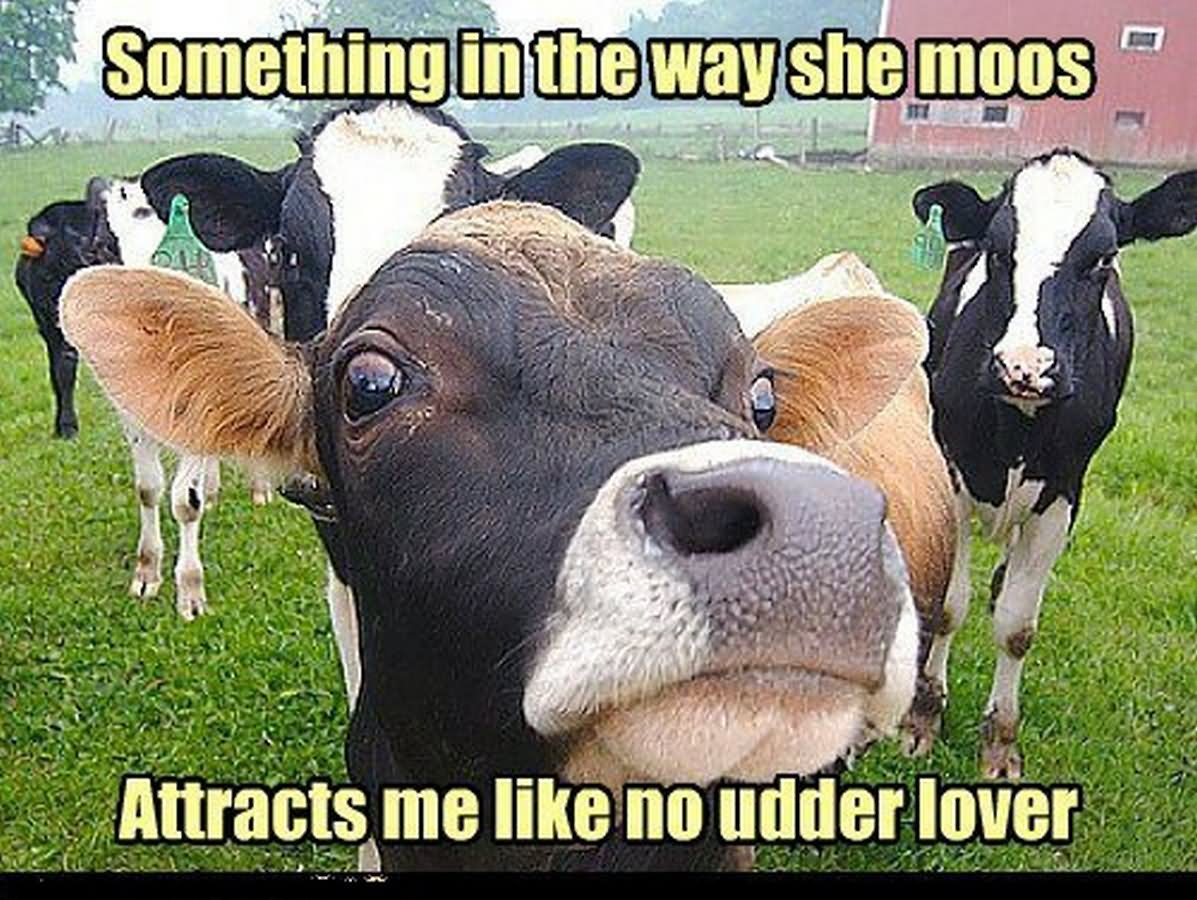
\includegraphics[width=0.75\textwidth]{will/example-image.jpg}
    \hfill
    \caption{An example image \citet{E-Cannon2022}}
    \label{fig:example-image}
\end{figure}

\vspace{-10mm}
\subsection{Example NUMBERED subsection (no * in environment)}
\vspace{-3mm}

Example equation \ref{eq:example-equation}.

\begin{equation}
    beef_{moo} = fear^{10}
    \label{eq:example-equation}
\end{equation}

Example list:

\begin{itemize}
    \item \(\bm{X} \in \mathbb{R}^{n \times p}\), a matrix containing the scrutinised data-points $\bm{x} \in \mathbb{R}^{p}$ from each sample,
    \item \textit{regression\textunderscore targets}, known as $\bm{\bar{y}}\in \mathbb{R}^n$, is a vector containing the regression targets for the samples (individually known as $\Bar{y}$), and
    \item \textit{class\textunderscore labels} $\in \{1,\dots,p\}$ which keeps track of which Gaussian each sample came from (a target for classification).
\end{itemize}

Example table \ref{table:1}

\begin{table}[!ht] % the [h] forces the table to be "here". This is quite a short document so LaTeX struggles to find a nice arrangement for the floats! Not normally needed
    \begin{center}
    
        \begin{tabular}{|l|c|c|} 
            \hline
            \textbf{learning\_rate} & \textbf{mse\_train} & \textbf{mse\_val} \\ 
            \hline
            1e-05&1.1254&1.1747\\
            \hline
            0.0001&0.31296&0.3012\\
            \hline
            0.001&0.095492&0.088045\\
            \hline
            0.01&0.046835&0.052905 \\
            \hline
            0.1&0.046534&0.052771\\
            \hline
            1&NaN&NaN \\
            \hline
        \end{tabular}
        \caption{Table of Mean Squared Difference from different learning rates.}
        \label{table:1}
            
    \end{center}
\end{table}

Example aligned equation:

\begin{align*}
    \mathcal{L}_c &= -ylog(\bar{y}) - (1-y)log(1-\bar{y})\\
    &= ylog(1+e^{-\bm{\hat{x}^T\theta}})-(1-y)log(\frac{e^{-\bm{\hat{x}^T\theta}}}{1+e^{-\bm{\hat{x}^T\theta}}})\\
    &=(y-y)log(1+e^{-\bm{\hat{x}^T\theta}})-(1-y)log(e^{-\bm{\hat{x}^T\theta}})+log(1+e^{-\bm{\hat{x}^T\theta}})\\
    &=(1-y)\bm{\hat{x}^T\theta}+log(1+e^{-\bm{\hat{x}^T\theta}})\\
    \Delta_{\bm{\theta}}\mathcal{L}_c &=(1-y)\bm{\hat{x}}-\frac{e^{-\bm{\hat{x}^T\theta}}}{1+e^{-\bm{\hat{x}^T\theta}}}\bm{\hat{x}}\\
    &=(1-y)\bm{\hat{x}}-(1-\bar{y})\bm{\hat{x}}\\
    &=\bm{\hat{x}}(\bar{y}-y)
\end{align*}

END OF TEMPLATE